\documentclass{article}
\usepackage{lipsum}
\usepackage[utf8]{inputenc}
\usepackage{braket}
\title{\underline {\textbf{Dimer solution of Hyperbolic Ising Model}}}
\author{Alapan Das}
\date{}%
\maketitle
%\usepackage{lipsum} 
\usepackage{biblatex} %Imports biblatex package
\addbibresource{bibtex.bib} %Import the bibliography file
\usepackage{appendix} % Package pour gérer les annexes
\usepackage{amsfonts}
\usepackage{xcolor}
\usepackage{amsmath}
\usepackage{graphicx}
\usepackage{physics}
\usepackage{hyperref}
\usepackage{url}

\hypersetup{
	colorlinks=true,
	linkcolor=blue,
	urlcolor=blue,
}

\begin{document}
	\maketitle 
	
     \textbf{Ising problem and Dimer Solution:} Our goal is to find the behavior of the spectrum of the Pfaffian matrix corresponding to the dimer model for the hyperbolic Ising model. In the presence of an external magnetic field, the usual dimer model mapping doesn't work as all the vertices can have any number of allowed edges. However, for a small magnetic field, we can expand the partition function as $Z=Z_0+hZ_1+h^2Z_2+...$. Here $Z_n$ includes exactly $n$ points that have odd numbers of edges. Generally speaking $Z_n=\sum_{x_1,x_2,...,x_n} \langle{\sigma(x_1)\sigma(x_2)...\sigma(x_n)}\rangle$. We can see from symmetry that the terms for odd $n$ are zero when the boundary condition is free, i.e. boundary spins can $\pm1$. In other words, we can not make a graph $\omega$ with only odd numbers of points having odd numbers of edges. A curve has to have two endpoints. So we get $Z=Z_0+h^2Z_2+h^4Z_4+....$. However, if we set all the boundary sites to $+1$ or $-1$ and look at $Z_{bulk}=Ze^{\beta h|\partial \Lambda|}$, we can take  $h^n$ terms where $n$ are odd as the paths end at the boundary. \\
     
     Having talked about the expansion, we see that our usual Fisher construction doesn't work as the points $x_i$ in $\langle{\sigma(x_1)\sigma(x_2)...\sigma(x_n)}\rangle$ has an odd number of edges but others have even. So we need to make the following modifications.\\
     
     
     \begin{center}
     	\includegraphics[scale=0.9]{Dimer.jpg}
     \end{center}
     
     This is the diagram of the modified dimer configuration to find magnetization at some point $x\in G$ of the graph. That is $\mu_{\Lambda, \beta}=\langle {\sigma(x)} \rangle =\text{Pfaff}(\tilde{A})$, where $\tilde{A}$ is the Pfaffian matrix for modified graph. The modification just includes adding three points (blue) around the $x$-triangle and flipping the rule of dimer matching for just the center $x$-triangle. These three points act like mediators between the point $x$ and the others to make their opposite dimer matching rule consistent. So, for the edges of this region, weights are $v_{e}=\tanh(\beta J_e)$, instead of its reciprocal, which is the case for all other edges. \\
     
     \vspace{0.5 cm}
     \pagebreak
     But this brings a global change to the Pfaffian orientation as we add an odd number of extra sites. As we have added three extra points, we may add one extra site at the boundary to keep the total number of points on the graph even.\\ 
     
     
     \begin{center}
     	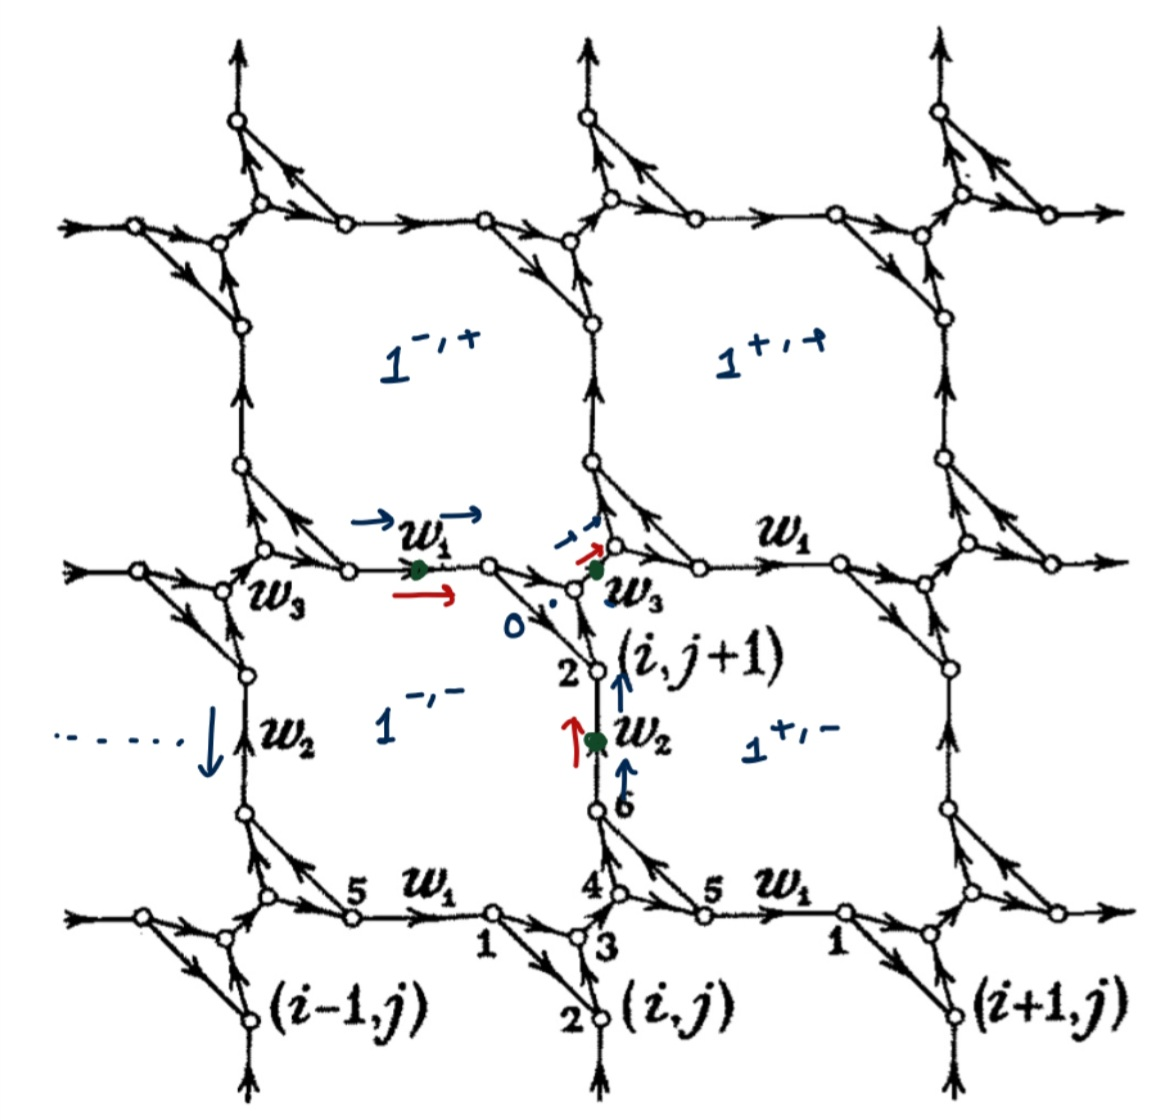
\includegraphics[scale=0.2]{pfaff mod.jpg}
     \end{center}\\

     
     This shows the orientation for the modified graph. The red lines (and the printed ones) are the original. The blue ones are after modification. So, there is a global orientation flip along a line as shown in the figure. This dimer configuration is not translationally invariant. We may join the extra legs at the corner or slightly modify the corners as well. There we take two points for one corner and do not do any Fisher construction. The dimer matching rule will be similar.\\ 
     
     We want to relate the spectrum of this matrix to the FK percolation as we can show that $=\mu^{+}_{\Lambda , T}=\langle{\sigma^{+}(x)}\rangle=\Phi^{w,p,2}[x \leftrightarrow \partial \Lambda ]$, where $\partial \Lambda$ is the boundary of the graph. This is equal to $\sum_{y \in \partial \Lambda} \langle{\sigma(x)\sigma(y)}\rangle$ for free boundary condtion.\\
     
     Here, $\Phi^{w,p,q}(\omega)=\prod_{e\in \omega} p^{\omega(e)}(1-p)^{1-\omega(e)}q^{Cl(w)}$, here $Cl$ stands for number of connected components, $w(e)=0,1$ for closed or open edges and $w$ stands for wired boundary condition, that is all the boundary sites are connected. Here, $p \equiv 1-e^{-2\beta J}$.\\
     
     When $p=0$, there is no connected cluster, and when $p=1$ there is only one connected cluster with probability 1. As the measure here is the number of connected clusters and not the total number of sites in those connected clusters, the FK measure $\Phi$ may not be monotonic in $p$. For amenable graphs however, we can show that $\Phi[0 \leftrightarrow \partial \Lambda ] \leq e^{-c_pn}$ similarly as we show for Bernoulli percolation.  \\
     
     We want to understand the dependence of the spectrum of the Pfaffian of modified Fisher graph for a hyperbolic lattice $(n,k)$. An important relation for any anti-symmetric matrix $A$ is $\partial_{\beta} \ln \text{Pf}(A)= \frac{1}{2}\Tr[A^{-1}\partial_{\beta}A]$, this may ease things. \\  
     
     \\
    \vspace{0.5 cm}
     \textbf{Constructing the hyperbolic lattice and builing it's Pfaffian matrix:} We get the eigenspecturm by building the hyperbolic lattice with Pfaffian orientation. Below we write down in detail how we build the hyperbolic lattice.\\
     
     1) $(n,3)$ Hyperbolic lattice satisfies this recurrence relation: Say $\alpha_g, \beta_g$ denotes the number of legged and legless nodes at the layer $g$. Then we can easily find the recurrence relation:$\alpha_{g+1}=(n-3)\alpha_g-\beta_{g} ; \beta_{g+1}=\beta_g$.\\
     
     2) For $n$ odd we give all the edges of the first layer clockwise orientations and for n even we set odd number of them in that manner. All the radial edges/layer connecting edges are given radially outward orientaions. And at last rest of the edges are given appropriate orientations in order to satisfy the requirement of Pfaffian orientation. \\
     
     3) For building $g$ edges all the internal vertices of the original graph are expanded with triangles. Also the layer connecting $\beta_{g}$ vertices of the last layer are also expanded in similar manner. But other vertices of the last layer are expanded to only two edges as they have degree $2$. \\
     
     4) As the constructed Pfaffian is an real anti-symmetric matrix, all it's eigenvalues are purely imaginary and comes in complex conjugate pairs with $\text{Pf}(A)=\prod \lambda_{\geq 0}$. \\
     
     This is the link to the python file for the written code: \href{https://github.com/ad1729-math/DP-Files/blob/main/Hyperbolic%20Pfaffian.py}{Hyperbolic Pfaffian}\\
     
     This file contains the code for the Pfaffian of a $(n,3)$ Hyperbolic lattice. Here we construct the lattice and it's expander graph followed by the construction of the Pfaffian, the eigenspectrums of which we plot for various temperature. \\
     
     \begin{center}
     	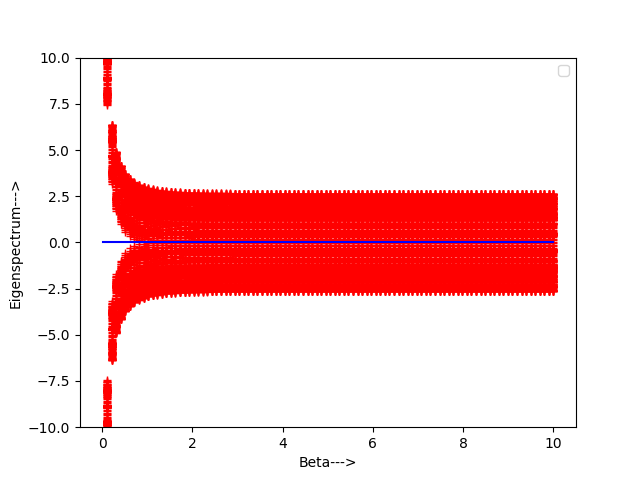
\includegraphics[scale=0.5]{Hyperbolic lattice eigenspectrum.png}\\
     	\textbf{Figure-1:} For $K=\beta J \in [0.01,10]$\\
     \end{center}
     
     For finite $g$ surely the partition function is analytic and no eigenvalue should be zero. But in $g \to \infty$ limit the smallest absolute eigenvalue touches the zero line. Explicitly written we get, $Z(\beta, J)=(2\sinh(\beta J))^{\xi(g)}\Delta(\beta, J)$.Where $\xi$ is the number of edges of the graph when there are $g$ layers. $\Delta$ is the Pfaffian generaing function. $\Delta(\beta, J)=\sum_{m \in \mathcal{M}}\prod_{e \in m} v_e$. Here, $v_e=\tanh(\beta J)^{-1}$ for the original edges and $v=1$ for expanded edges.\\
     
     This can be seen that when $T \to \infty$, $Z \to 2^{\xi(g)}$ and for $T \to 0$, $Z \to (2^{\xi(n)}P(g))$ where $P(g)$ is number of perfect matchings for the expander graph.\\
     
     \begin{center}
     	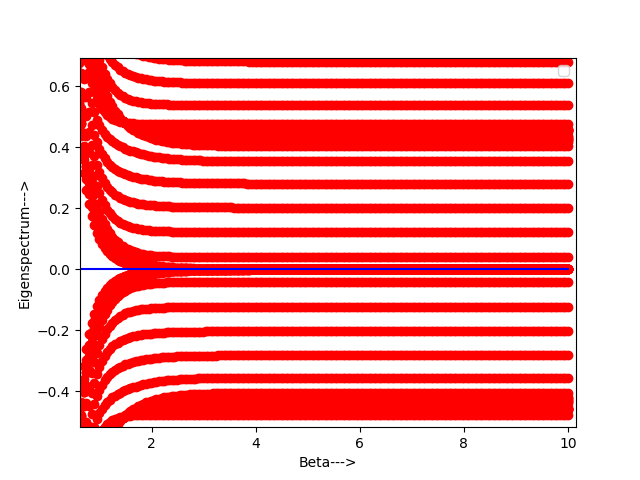
\includegraphics[scale=0.5]{Hyperbolic lattice eigenspectrum 1.png}\\
     	\textbf{Figure-2:} For $K=\beta J \in [0.01,2]$\\
     \end{center}
     
     \begin{center}
     	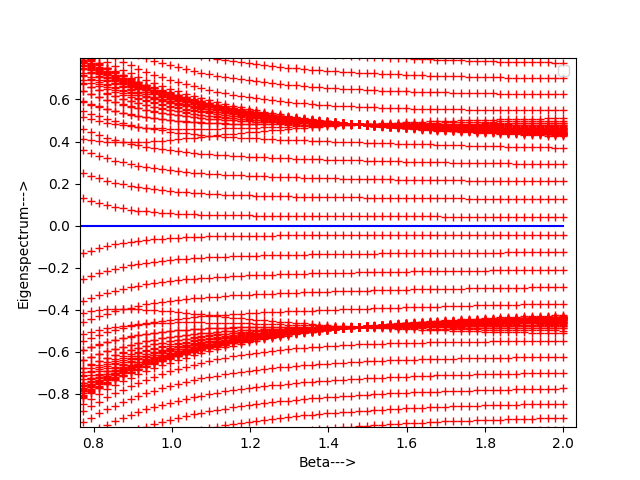
\includegraphics[scale=0.5]{Crossings.png}\\
     	\textbf{Figure-3:} Observation of crossings\\
     \end{center}
   
     \begin{center}
     	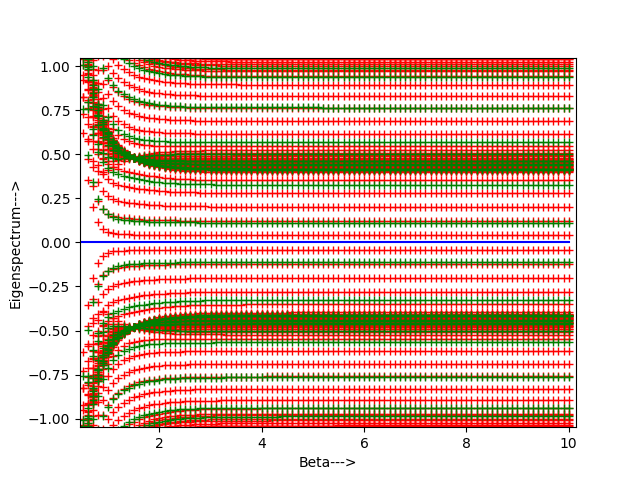
\includegraphics[scale=0.5]{Crossing 2.png}\\
     	\textbf{Figure-4:} Observation of crossings for $g=3$ (red) and $g=2$ (green).\\
     \end{center}
     \vspace{0.2 cm}
     \textbf{Comment:} There are two crossings at two different $\beta$. Those may indicate two phase transitions.\\
     
     Below we plot $\ln (\text{Pf})(\beta, J)=\prod \lambda_{\geq 0}$ as function of $K=\beta J$ for $K \in [0.01,10]$. We see that the dimer partition function goes to the $T=0$ at around $K=2$. Green and red curves are for $2$ and $1$ layers respectively.\\
     \begin{center}
     	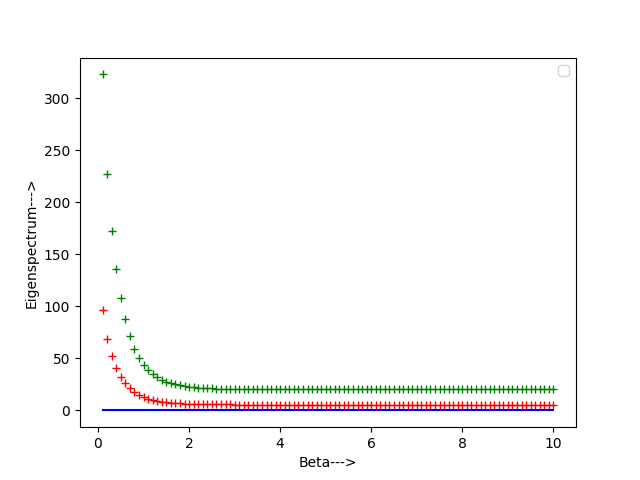
\includegraphics[scale=0.5]{Log Pfaffian.png}\\
     	\textbf{Figure-:} $\ln(\text{Pf})$ as a function of $K=\beta J$\\
     \end{center}

\end{document}